\graphicspath{{forms/asy/}}


\section{Vector Fields \& Differential Forms}\label{chap:forms}

\begin{minipage}[t]{0.75\linewidth}\vspace{-10pt}
	In preparation for our study of surfaces, we further develop the notion of a tangent vector. To permit easy differentiation, throughout this section all functions are assumed to be \emph{smooth} (infinitely differentiable) and $U\subseteq\R^n$ will denote a \emph{\textcolor{blue}{connected open set}}: (informally) a region consisting of a single piece without edge points. As previously, $n$ will always be 1, 2 or 3: when $n=1$, $U=(a,b)$ is an open interval; the picture illustrates $n=2$.
\end{minipage}
\hfill
\begin{minipage}[t]{0.24\linewidth}\vspace{-5pt}
	\flushright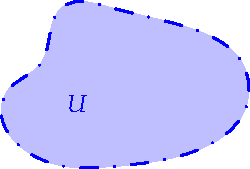
\includegraphics[scale=0.95]{forms-open}
\end{minipage}


\subsection{Directional Derivatives, Tangent Vectors \& Vector Fields}\label{sec:vfield}

First recall some basic objects and facts from elementary multivariable calculus.

\begin{defn}{}{}
	The \emph{gradient} of $f:U\subseteq\R^n\to\R$ is the function $\nabla f:U\to\R^n$ defined by
	\[
		\nabla f(\lst xn)=\left(\partials[f]{x_1},\ldots,\partials[f]{x_n}\right)
	\]
	Given a point $p\in U$, a vector $\vv=(\lst{v}{n})\in \R^n$, and a function $f:U\to\R$, the \emph{directional derivative} of $f$ at $p$ in the direction $\vv$ is the \emph{scalar}
	\[
		D_\vv f(p):=\sum_{k=1}^nv_k\partialsat[f]{x_k}{p} =\vv\cdot\bigl(\nabla f(p)\bigr)
	\]
\end{defn}


\begin{example}{}{}
	Suppose $f(x,y,z)=x^2-z\cos y$, $p=(1,\pi,0)$, and $\vv=(3,5,1)$. Then
	\[
		\nabla f=\threevec{2x}{z\sin y}{-\cos z} \implies D_\vv f(p)=\threevec 351\cdot\threevec{2}{0}{1} =7
	\]
\end{example}

The directional derivative describes the rate of change of the value of $f$ in a given direction.

\begin{lemm}{}{dirderiv}
\exstart By the chain rule, if $\textcolor{blue}{\vx(t)}$ is a curve such that $\vx(0)=p$ and $\vx'(0)=\vv$, then
\begin{enumerate}\setcounter{enumi}{1}
  \begin{minipage}[t]{0.62\linewidth}\vspace{-12pt}
  	\item[]
  \[
  	\diffat t{t=0}f\bigl(\vx(t)\bigr) =\sum_{k=1}^n\partialsat[f]{x_k}{p}x'_k(0) %=D_\vv f\bigl(\vx(0)\bigr)
  	=D_\vv f(p)
  \]
  is the rate of change of $f$ at $p$ \emph{as one travels along the curve}.
	\item If $t$ is small, then $f(p+t\vv)\approx f(p)+D_{\vv}f(p)\,t$.
  \item If $\vv$ is a unit vector making angle $\theta$ with $\nabla f(p)$, then
  \[D_{\vv}f(p)=\vv\cdot\nabla f(p)=\Nm{\nabla f(p)}\cos\theta\]
  \end{minipage}
  \hfill
  \begin{minipage}[t]{0.35\linewidth}\vspace{-8pt}
  	\flushright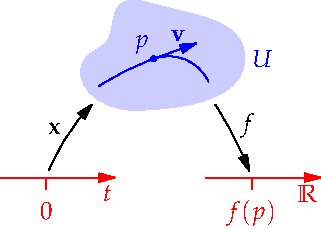
\includegraphics{forms-dderiv}
  \end{minipage}
  \medbreak
  is maximal when $\vv$ points in the same direction as $\nabla f(p)$. Otherwise said, $\nabla f(p)$ points in the direction of greatest increase of $f$ at $p$; its magnitude measures the rate of change.
\end{enumerate}
\end{lemm}


\goodbreak


By placing the function $f$ at the end of the directional derivative, we are tempted to create an \emph{operator}
\[
	\at{D_\vv}{p}=\sum_{k=1}^nv_k\partialsat{x_k}{p}
\]
which takes a \emph{function} $f:U\to\R$ and returns the \emph{scalar} $D_\vv f(p)$.
This operator is a map (function) from the set of smooth functions $f:U\to\R$ to the real numbers. It is even more tempting to drop the point $p$ and allow the components of $\vv$ to be \emph{smooth functions.} This yields a new definition of an old concept.

\begin{defn}{}{vfield}
	The set of directional derivative operators $\at{D_\vv}{p}$ is the \emph{tangent space} $T_p\R^n$ at $p\in\R^n$.\par
	A \emph{vector field} $v$ on $U\subseteq\R^n$ is a smooth choice for each $p\in U$ of an element of $T_p\R^n$: that is
	\[
		v=\sum_{k=1}^nv_k\partials{x_k}\ \text{ where each $v_k:U\to\R$ is smooth}
	\]
	Each operator $\partials{x_k}$ is termed a \emph{co-ordinate vector field.}\par
	If $f:U\to\R$ is smooth, we write $v[f]=\sum v_k\partials[f]{x_k}$ for the result of applying the vector field $v$ to $f$; this is itself a smooth function $v[f]:U\to\R$.
\end{defn}

Each tangent space $T_p\R^n$ is a vector space, with natural basis $\smash[b]{\partials{x_1}\big|_p,\ldots,\partials{x_n}\big|_p}$. In this brave new world, a tangent vector $v_p=\sum v_k\partials{x_k}\big|_p$ corresponds to our previous notion $\vv_p=(v_1,\ldots,v_n)$. While this might seem artificially complicated, the rational is simple: the purpose of tangent vectors is to measure how functions change in given directions (Lemma \ref{lemm:dirderiv}!).


\begin{examples}{}{}
	\exstart The vector field $v=3x\partials{x}+2xz\partials{y}-x\partials{z}$ on $\R^3$ corresponds to the vector-valued function $\vv(x,y,z)=(3x,2xz,-x)$. Given $f(x,y,z)=xy^2+z$, we have
	\[
		v[f]=3x\partials[f]{x}+2xz\partials[f]{y}-x\partials[f]{z}=6x^2y+2x^3z-x
	\]
	which, as expected, is a smooth function $v[f]:\R^3\to\R$.
	
	\begin{enumerate}\setcounter{enumi}{1}
		\item Suppose, in $\R^2$, that we are given a \emph{vector field} $v=y^2\partials{x}-x\partials{y}$, a \emph{function} $f(x,y)=x^2y$, and a \emph{point} $p=(2,-1)$. These may be combined in various ways, for instance:
		\[
			\def\arraystretch{1.7}
			\begin{array}{@{}l@{\qquad}l}
				\text{\emph{Vector field on $\R^2$}} & \displaystyle fv=x^2y\left(y^2\partials{x}-x\partials{y}\right) =x^2y^3\partials{x}-x^3y\partials{y} \\
	 			\text{\emph{Tangent vector}} & \displaystyle (fv)(p)=f(p) v_p=-4\partialsat{x}p+8\partialsat{y}p \in T_p\R^2 \\
				\text{\emph{Function} $\R^2\to\R$} & \displaystyle v[f]=y^2\partials{x}(x^2y)-x\partials{y}(x^2y)=2xy^3-x^3 \\
	 			\text{\emph{Number}} & \displaystyle \bigl(v[f]\bigr)(p) =-4-8=-12
			\end{array}
		\]
		Note the use of different brackets! Note also that $fv$ denotes the vector field obtained by \emph{multiplying} $v$ by the \emph{value} of $f$ at each point. It does \emph{not} mean \emph{apply the function $f$ to the vector field $v$,} which makes no sense!
	\end{enumerate}
\end{examples}

\goodbreak

Here are the basic rules of computation for vector fields. These are all essentially trivial if you take $v=\sum v_k\partials{x_k}$, etc., as in Definition \ref{defn:vfield}. Just be careful with notation!

\begin{lemm}{}{vfieldrules}
	Let $v,w$ be vector fields on $U$, let $f,g:U\to\R$ be smooth, and $a,b\in\R$ constant. Then,
	\begin{enumerate}
	  \item $fv+gw$ is a vector field: at each $p\in U$, $(fv+gw)(p):=f(p)v_p+g(p)w_p$
		\item Vector fields act linearly on smooth functions: \ $v[af+bg]=av[f]+bv[g]$
		\item (Leibniz rule)\ \ Vector fields obey a product rule: \ $v[fg]=fv[g]+gv[f]$
	\end{enumerate} 
\end{lemm}

\begin{example}{Polar Co-ordinates}{polar}
	Let $U$ be the plane without the non-positive $x$-axis. On $U$, the standard \emph{rectangular co-ordinates} $(x,y)$ are related to the \emph{polar co-ordinates} $(r,\theta)$ via
	\[
		\begin{cases}
			x=r\cos\theta\\
			y=r\sin\theta
		\end{cases}
		\quad\leftrightsquigarrow\quad
		\begin{cases}
			r=\sqrt{x^2+y^2}\\
			\theta=\tan^{-1}\frac yx\quad (\text{or $\pm\frac\pi 2$ if $x=0$})
		\end{cases}
	\]
	The chain rule tells us that the co-ordinate vector fields $\partials x,\partials y,\partials r,\partials\theta$ are related via\par
	\begin{minipage}[t]{0.6\linewidth}\vspace{-10pt}
		\begin{gather*}
			\begin{aligned}
				\partials r&=\partials[x]{r}\partials x+\partials[y]{r}\partials{y} =\cos\theta\partials x+\sin\theta\partials y\\
				&=\frac 1{\sqrt{x^2+y^2}}\left(x\partials x+y\partials y\right)
			\end{aligned}
			\\[5pt]
			\begin{aligned}
				\partials\theta&=\partials[x]{\theta}\partials x+\partials[y]{\theta}\partials{y} =-r\sin\theta\partials x+r\cos\theta\partials y\\
				&=-y\partials x+x\partials y
			\end{aligned}
		\end{gather*}
	\end{minipage}
	\hfill
	\begin{minipage}[t]{0.39\linewidth}\vspace{0pt}
		\flushright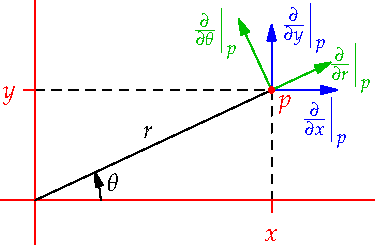
\includegraphics{forms-polar}
	\end{minipage}
	\bigbreak
	At $p$, these point in the direction of maximal increase for the corresponding co-ordinate.\smallbreak
	We could similarly compute $\partials x$ and $\partials y$ by differentiating. For variety, we instead use linear algebra:
	\begin{align*}
		\twovec{\partials r}{\partials\theta}
		=
		\begin{pmatrix}
			\cos\theta&\sin\theta\\
			-r\sin\theta&r\cos\theta
		\end{pmatrix}
		\twovec{\partials x}{\partials y}
		&\implies
		\twovec{\partials x}{\partials y}
		=
		\frac 1r
		\begin{pmatrix}
			r\cos\theta&-\sin\theta\\
			r\sin\theta&\cos\theta
		\end{pmatrix}
		\twovec{\partials r}{\partials\theta}\\
		&\implies
		\begin{cases}
			\displaystyle \partials x=\cos\theta\partials r-\frac{\sin\theta}r\partials\theta\\[5pt]
			\displaystyle \partials y=\sin\theta\partials r+\frac{\cos\theta}r\partials\theta
		\end{cases}
	\end{align*}
	The first matrix is the familiar \emph{Jacobian} $\partials[(x,y)]{(r,\theta)}$ from multivariable calculus.
	Strictly, we are viewing $U$ as subsets of \emph{two different versions of $\R^2$}:
	\begin{itemize}
	  \item In rectangular co-ordinates, $U=\R^2\setminus\{(x,0):x\le 0\}$ is a cut plane.
	  \item In polar co-ordinates, $U=(0,\infty)\times(-\pi,\pi)$ is an infinite open rectangle.
	\end{itemize}
	In practice, particularly since we are so familiar with polar co-ordinates, it is easier to stick to the first interpretation and draw all four co-ordinate tangent vectors on the same picture.
\end{example}


\clearpage


\begin{exercises}
	\exstart You are given the following vector fields and functions
		\begin{align*}
			&u=7\partials{x}-3\partials{y}
			&&v=x\partials{x}+2y\partials{y}
			&&w=\sin x\partials{x}-2\cos x\partials{y}\\
			&f(x,y)=xy^2
			&&g(x,y)=-y
			&&
		\end{align*}
		
	\begin{enumerate}\setcounter{enumi}{1}
  	\item[] Compute the \emph{functions}:
  	\begin{enumerate}
    	\item \makebox[120pt][l]{$u[f]$\hfill (b)}\lstsp \makebox[120pt][l]{$v[f]$\hfill (c)}\lstsp $w[f]$
    	\setcounter{enumii}{3}
    	\item \makebox[120pt][l]{$v[fg]$\hfill (e)}\lstsp \makebox[120pt][l]{$fu[g]$\hfill (f)}\lstsp $v\bigl[w[g]\bigr]$
  	\end{enumerate}
  
  
	  \item Revisit Example \ref{ex:polar} on polar co-ordinates.
	  \begin{enumerate}
	    \item Use the chain rule to compute $\partials x$ and $\partials y$ directly in terms of $r,\theta,\partials r$ and $\partials\theta$ and verify that you obtain the same expressions as the linear algebra approach.
	    \item Suppose $T_p\R^2$ is equipped with the standard dot product so that \smash[b]{$\partialsat xp$ and $\partialsat yp$} are considered orthonormal.
	    \begin{enumerate}
	      \item Show that $\partialsat rp$ and $\partialsat\theta p$ are perpendicular.
	      \item What are the lengths of $\partialsat rp$ and $\partialsat\theta p$?
	  	\end{enumerate}
	  \end{enumerate}
  
  
	  \item\label{exs:spherical} Consider the spherical polar co-ordinate system
	  \[
	  	\begin{cases}
				x=r\cos\theta\cos\phi\\
	  		y=r\sin\theta\cos\phi\\
	  		z=r\sin\phi
	  	\end{cases}
	  	\qquad
	  	\text{where $r>0$, \ $0<\theta<2\pi$ and $-\frac\pi 2<\phi<\frac\pi 2$}
	  \]
	  Show that
	  \[
	  	\partials r=\frac 1r\left(x\partials x+y\partials y+z\partials z\right)
	  \]
	  
	  
	  \item Prove the Leibniz rule (Lemma \ref{lemm:vfieldrules} part 3).
	  
	  
	 	\item If $f,g,h$ are smooth functions and $v$ is a vector field, expand $v[fgh]$ using the Leibniz rule.
	  
	  
	  \item Let $s=x^2-y^2$ and $t=2xy$. Compute $\partials s,\partials t$ in terms of $\partials x$ and $\partials y$.\par
	  (\emph{Hint: use the chain rule to find $\partials x$ and $\partials y$, then invert the Jacobian})
	  
	\end{enumerate}
\end{exercises}

\clearpage



\subsection{Differential 1-forms}\label{sec:1form}

Make sure you are comfortable with vector fields \emph{before} you tackle this section and the next! There is a lot of new notation to get used to here, but with a little practice it is very easy to use. 

\begin{defn}{}{}
	Let $(x_1,\ldots,x_n)$ be co-ordinates on $U\subseteq\R^n$ and $p\in U$. The \emph{(co-ordinate) 1-form $\dx_k$ at $p$} is the \emph{linear map\footnotemark} $\dx_k:T_p\R^n\to\R$ defined by
	\[
		\dx_k\left(\partialsat{x_j}{p}\right)=\delta_{jk}=
		\begin{cases}
			1&j=k\\
			0&j\neq k
		\end{cases}
	\]
	A \emph{1-form} $\alpha=\sum\limits_{k=1}^n a_k\,\dx_k$ on $U$ is a smooth assignment ($a_k:U\to\R$ \emph{smooth}) of 1-forms.\par
	If $v$ is a vector field on $U$, we write $\alpha(v)$ for the \emph{function} $U\to\R$ obtained by mapping $p\mapsto\alpha(v_p)$.
\end{defn}

\footnotetext{For those who've met dual vector spaces in linear algebra, the set of 1-forms at $p$ is the \emph{cotangent space} $T_p^*\R^n$, or the space of \emph{covectors.} At each $p$, $\{\dx_1,\ldots,\dx_n\}$ is the \emph{dual basis} to $\smash[b]{\bigl\{\partialsat{x_1}p,\ldots,\partialsat{x_n}p\bigr\}}$.}


\begin{examples}{}{}
	\exstart Consider the vector field $v=xy\partials x-2\partials y$ on $\R^2$. At each $p\in\R^2$, the components $xy$ and $-2$ are \emph{scalars} and thus ignored by the linear map $\dx:T_p\R^2\to\R$. We therefore obtain a \emph{function} $\dx(v):\R^2\to\R$
	\[
		\dx(v)=\dx\left(xy\partials x-2\partials y\right)=xy\,\dx\left(\partials x\right)-2\,\dx\left(\partials y\right) =xy
	\]
	\begin{enumerate}\setcounter{enumi}{1}
	  \item Again on $\R^2$, let $\alpha=2x\,\dx+\dy$ and $v=x^2y\partials x-e^{xy}\partials y$. Then
		\[
			\alpha(v)=(2x\,\dx+\dy)\left(x^2y\partials x-e^{xy}\partials y\right) =2x^3y-e^{xy}
		\]
	\end{enumerate}
\end{examples}

\phantomsection\label{pg:formlinearfunction}
Remember that a 1-form $\alpha$ is linear \emph{when restricted to each tangent space} $T_p\R^n$: if $v_p\in T_p\R^n$ and $f:U\to\R^n$, we obtain a \emph{real number}
\[
	\alpha_p\bigl(f(p)v_p\bigr)=f(p)\alpha_p\bigl(v_p\bigr)\in\R
\]
by pointwise multiplication by the value of $f$. Taken over all points $p$, this means that scalar \emph{functions} come straight through a 1-form: if $v$ is a vector field on $U$, then
\[
	\alpha(fv)=f\alpha(v)
\] 


\begin{defn}{}{extderiv}
	Let $f:U\to\R$ be \emph{smooth}. The \emph{exterior derivative} of $f$ is the 1-form
	\[
		\df=\sum_{k=1}^n\partials[f]{x_k}\,\dx_k=\partials[f]{x_1}\dx_1+\cdots+\partials[f]{x_n}\dx_n
	\]
	If a 1-form is the exterior derivative of a function, we say that it is \emph{exact.}
\end{defn}
\clearpage
Our approach essentially splits a derivative into two pieces: for each $k$, we have $\smash{\df\left(\partials{x_k}\right)=\partials[f]{x_k}}$.
Moreover, since a linear map $(\df_p:T_p\R^n\to\R)$ is determined by what it does to a basis, the exterior derivative $\df$ is the \emph{unique} 1-form with the property that $\df(v)=v[f]$ for all vector fields $v$ on $U$. This says that the definition is \emph{co-ordinate independent} (does not depend on $x_1,\ldots,x_n$).


\begin{examples}{}{}
	\exstart Let $f(x,y)=x^2y$, then $\df=\alpha=2xy\,\dx+x^2\dy$. As a sanity check, consider a general vector field $v=a\partials x+b\partials y$ (remember that $a,b$ are smooth functions!) and compute 
	\[
		\df(v)=2axy+bx^2=v[x^2y]
	\]
	\begin{enumerate}\setcounter{enumi}{1}
	  \item If $\alpha=4xy^2\,\dx+(4x^2y+1)\,\dy=f_x\,\dx+f_y\,\dy$ is exact, then `partial integration' forces
	  \[
	  	f(x,y)=\int 4xy^2\,\dx=2x^2y^2+g(y) =\int 4x^2y+1\,\dy=2x^2y^2+y+h(x)
	  \]
	  for some functions $g,h$. Plainly $g,h$ must be constant and $\alpha=\D(2x^2y^2+y)$.
	  
	  \item We could a similar game to see that $\alpha=3x^2y\,\dx+2\,\dy$ is \emph{not} exact on $\R^2$. Alternatively, note that if $\alpha=\df=f_x\,\dx+f_y\,\dy$, we obtain a contradiction by observing that the mixed partial derivative is simultaneously
	  \[
	  	3x^2=\partials[f_x]{y}=f_{xy}=f_{yx}=\partials[f_y]{x}=0
	  \]
	  See Exercise \ref{exs:exactclosed} for the general result.
	\end{enumerate}
\end{examples}


\begin{lemm}{}{formeasy}
	If $f,g$ are smooth functions, then
	\begin{enumerate}%\itemsep0pt
		\item $\D(f+g)=\df+\dg$
		\item $\D(fg)=f\,\dg+g\,\df$
		\item $\df=0\iff f$ is a constant function
	\end{enumerate}
\end{lemm}

\begin{proof}
	These follow straight from the definition of $\df$. For instance
	\[
		\df=0\iff \partials[f]{x_j}=\df\left(\partials{x_j}\right)=0\text{ for all }j=1,\ldots,n \iff f\text{ is constant} \tag*{\qedhere}
	\]
\end{proof}

\begin{example*}{\ref*{ex:polar} cont}{}
	The exterior derivative and part 2 of the Lemma make it easy to compute the relationship between the 1-forms $\dx,\dy,\dr,\dth$:
	\[
		\begin{cases}
			x=r\cos\theta\\
			y=r\sin\theta
		\end{cases}
		\implies 
		\begin{cases}
			\dx=\cos\theta\,\dr-r\sin\theta\,\dth\\
			\dy=\sin\theta\,\dr+r\cos\theta\,\dth
		\end{cases}
		\implies
		\begin{cases}
			\dr=\frac 1r(x\,\dx+y\,\dy)\\
			\dth=\frac 1{r^2}(-y\,\dx+x\,\dy)
		\end{cases}
	\]
	We may also verify directly that the dual basis relations hold; for instance,
	\begin{align*}
	% \dx\left(\partials x\right) &=\left(\cos\theta\,\dr-r\sin\theta\,\dth\right)\left(\cos\theta\partials r-\frac{\sin\theta}r\partials\theta\right)\\
	% &=\cos^2\theta\,\dr\left(\partials r\right) -\frac{\cos\theta\sin\theta}r\,\dr\left(\partials\theta\right) -r\sin\theta\cos\theta\,\dth\left(\partials r\right) +\sin^2\theta\,\dth\left(\partials\theta\right)=1
		\dr\left(\partials r\right) &=\frac 1r(x\,\dx+y\,\dy)\left(\cos\theta\partials x+\sin\theta\partials y\right) =\frac 1r(x\cos\theta+y\sin\theta)\\
		&=\cos^2\!\theta+\sin^2\!\theta=1
	\end{align*}
\end{example*}

\vfil\goodbreak



\boldsubsubsection{Elementary Calculus \& Line Integrals}

It is worth reviewing some staples from basic calculus in our new language.\smallbreak
If $f:\R\to\R$ is differentiable, then its exterior derivative $\df=f'(x)\,\dx$ feels familiar.\footnote{Consider the equivalence of notations $\diff[f]{x}=f'(x)$, linear approximations (differentials) \& integration by substitution.} To make sense of this as a relation between 1-forms we need \emph{vector fields}: the derivative of $f$ isn't the ratio of two 1-forms, rather it is the application of the 1-form $\df$ to the vector field $\diff x$:
\[
	\diff[f]{x}=\diff x[f]=\df\left(\diff x\right)
\]
Vector fields in $\R$ are written with a straight $\D$ rather than partial $\partial$ since there is only one direction in which to differentiate!\smallbreak

You've seen 1-forms before when integrating: we integrate 1-forms over oriented curves.

\begin{defn}{}{}
Let $\alpha$ be a 1-form on $U\subseteq\R^n$ and suppose $\vx:[a,b]\to U$ parametrizes a smooth curve $C$. Our usual identification (Definition \ref{defn:vfield}) produces the \emph{tangent vector field}
\[\vx'(t)=x_1'(t)\partials{x_1}+\cdots +x_n'(t)\partials{x_n}\]
along the curve. Now define the integral of $\alpha$ along $C$ by
\[\int_{C}\alpha:=\int_a^b\alpha\bigl(\vx(t)\bigr)\,\dt=\int_a^b\alpha\left(x_1'(t)\partials{x_1}+\cdots +x_n'(t)\partials{x_n}\right)\dt\]
\end{defn}


\begin{examples}{}{}
	\exstart We integrate $\alpha=x\,\dy$ over the unit-circle $\vx(t)=(\cos t,\sin t)$ counter-clockwise. Differentiate to obtain the tangent vector field $\vx'(t)=-\sin t\partials{x}+\cos t\partials{y}$, then
	\[
		\int_{C}\alpha=\int_0^{2\pi}\alpha\bigl(\vx'(t)\bigr)\,\dt \int_0^{2\pi}\cos^2t\,\dt =\frac 12\int_0^{2\pi}1+\cos 2t\,\dt=\pi
	\]
	\begin{enumerate}\setcounter{enumi}{1}
		\item Integrate $\alpha=y^2\,\dx-x^2\,\dy$ over the curve $\vx(t)=(t,t^2)$ between $(0,0)$ and $(1,1)$:
		\begin{align*}
			\int_{C}\alpha&=\int_0^1\alpha\bigl(\vx'(t)\bigr)\,\dt = \int_0^1\alpha\left(\partials x+2t\partials y\right)\,\dt =\int_0^1\left(\bigl(y(t)\bigr)^2-2t\bigl(x(t)\bigr)^2\right)\,\dt\\
			&=\int_0^1t^4-2t^3\,\dt=\frac 15-\frac 12=-\frac 3{10}
		\end{align*}
	\end{enumerate}
\end{examples}

\begin{lemm}{}{lineintparam}
	The integral of a 1-form along a curve is independent of the choice of (orientation-preserving) parametrization.
\end{lemm}

Otherwise said, if $\vx(t)=\vy\bigl(s(t)\bigr)$ parametrizes the same curve where $s'(t)>0$, then
\[
	\int_a^b\alpha\bigl(\vx'(t)\bigr)\,\dt=\int_{s(a)}^{s(b)}\alpha\bigl(\vy'(s)\bigr)\,\ds
\]
The proof is an easy exercise in interpreting old material (the chain rule/substitution).\smallbreak

Our final result from elementary calculus shows that integrals of exact forms are independent of path. This is essentially the fundamental theorem of calculus for curves.

\begin{thm}{Fundamental Theorem of Line Integrals}{exact}
	If $f$ is a function on $U\subseteq\R^2$ and $C$ is a curve in $U$, then the integral of $\df$ depends only on the values of $f$ at the endpoints of $C$:
	\[
		\int_{C}\,\df=f\bigl(\text{end of $C$}\bigr)-f\bigl(\text{start of $C$}\bigr)
	\]
	The converse also holds: if $\int_C\alpha$ is independent of path, then $\alpha$ is exact.
\end{thm}

\begin{proof}
	Suppose $\vx:[a,b]\to U$ parametrizes $C$, then
	\begin{align*}
		\int_{C}\,\df&=\int_a^b\df(\vx')\,\dt=\int_a^b\vx'[f]\,\dt =\int_a^b\left(x_1'(t)\partials[f]{x_1}+\cdots+x_n'(t)\partials[f]{x_n}\right)\,\dt\\
		&=\int_a^b\diff{t}\bigl(f(\vx(t))\bigr)\,\dt =f\bigl(\vx(b)\bigr)-f\bigl(\vx(a)\bigr)
	\end{align*}
	The converse is sketched in an exercise.
\end{proof}

In elementary multivariable calculus this result was written $\int_C\nabla f\cdot\dvx=f\bigl(\vx(b)\bigr)-f\bigl(\vx(b)\bigr)$ which comports with our new notation when we view $\dvx$ as a vector of 1-forms:
\[
	\nabla f\cdot\dvx=\threevec{\partials[f]{x_1}}{\vdots}{\partials[f]{x_n}}\cdot\threevec{\dx_1}{\vdots}{\dx_n}=\partials[f]{x_1}\dx_1+\cdots+\partials[f]{x_n}\dx_n =\df
\]
The exterior derivative $\df$ is just the gradient in disguise!

\begin{example}{}{}
	If $\alpha=\cos(xy)(y\,\dx+x\,\dy)$, find the integral of $\alpha$ over any curve $C$ joining the points $\left(\pi,\frac 13\right)$ and $\left(\frac 12,\pi\right)$. Since $\alpha=\D\sin(xy)$ is exact on $\R^2$, we see that
	\[
		\int_C\alpha=\sin(xy)\Bigr|_{\left(\pi,\frac 13\right)}^{\left(\frac 12,\pi\right)}=\sin\frac \pi 2-\sin\frac \pi 3=1-\frac{\sqrt 3}2
	\]
\end{example}


\boldsubsubsection{Summary}

\begin{itemize}\itemsep0pt
  \item Tangent vectors \& vector fields encode \emph{directional derivatives,} measuring how functions change in given directions.
  
  \item Vector fields and 1-forms break standard derivatives into two pieces: the result is a more flexible and extensible language for describing familiar results from multi-variable calculus.
\end{itemize}

The real pay-off comes once our new language is applied to surfaces and higher-dimensional objects. Here is a précis. A parametrized surface is a function $\vx:U\subseteq\R^2\to\E^3$; its exterior derivative $\dvx$ is a vector-valued 1-form which, at each point $p\in U$, describes a \emph{linear map} between tangent spaces
\[
	\dvx_p:T_p\R^2\to T_{\vx(p)}\E^3
\]
which maps the co-ordinate fields $\partials x,\partials y$ on $U$ to corresponding vector fields \emph{tangent to the surface.}

\clearpage

% \begin{aside}
% {\bf Exact 1-forms and integration---SCRAP!!!}\ \ An \emph{exact} 1-form on $U$ is a 1-form $\alpha$ that may be written $\D f$ for some smooth function $U\to\R$. Theorem \ref{thm:exact} says that the integral of an exact 1-form between two points is independent of the path you integrate over. Moreover, the integral of an exact 1-form over any closed curve is zero. There are times when you have to be careful when integrating, for it can seem like you have an exact 1-form when in fact you do not. Consider the 1-form $\D\theta$ on $U=\R^2\setminus\{0\}$ ($\D\theta$ is undefined at zero). This appears to be exact, being the exterior derivative of the co-ordinate function $\theta:U\to\R$. However $\theta$ is not a smooth function on the whole of $U$: after one revolution, $\theta$ has increased from 0 to $2\pi$ thus, in order to make $\theta$ a \emph{function} you are forced to choose a branch line where it is discontinuous and therefore not differentiable (let alone smooth). $\D\theta$ is therefore \emph{not exact}. Indeed, if $\gamma$ is the unit circle, then
% \[\int_\gamma\D\theta=2\pi.\]
% However if the closed curve $\gamma$ is chosen so that it does not circuit the origin (and doesn't self-intersect), then $\D\theta$ is exact on the domain of $\gamma$ and $\int_\gamma\D\theta=0$ 
% %\centering\includegraphics{17}
% 
% The requirement that $\gamma$ has no self-intersections can be dropped. Indeed we have the following result: if $\gamma$ is a closed curve in $\R^2\setminus\{0\}$ which orbits the origin $n$ times counter-clockwise then $\int_\gamma\D\theta=2\pi n$.
% \end{aside}



\begin{exercises}
	\exstart In $\R^2$, let $\alpha=2y\,\dx-3\,\dy$ and $v=3x^2\partials{x}+\partials{y}$. Compute $\alpha(v)$, and $v\bigl[\alpha(v)\bigr]$.
	\begin{enumerate}\setcounter{enumi}{1}
  	\item On $\R^3$, suppose $f(x,y,z)=x^2\cos(yz)$ and $v=e^x\partials x+2y\partials z$. Verify that $\df(v)=v[f]$.
  
  
 		\item Find $\dr$ directly by taking the exterior derivative of the equation $r^2=x^2+y^2$.
  
  
  	\item Prove parts 1 and 2 of Lemma \ref{lemm:formeasy}.
  
  
  	\item Continuing Example \ref{ex:polar}, verify that $\smash{\dth\left(\partials\theta\right)=1}$, and $\smash[b]{\dr\left(\partials\theta\right)=0=\dth\left(\partials r\right)}$.
  
	
  	\item\label{exs:exactclosed} Suppose that $\alpha=\sum a_k\,\dx_k$ is exact. Prove that $\smash{\partials[a_k]{x_j}=\partials[a_j]{x_k}}$ for all $j,k$.
  
  
  	\item Decide whether the 1-forms $\alpha$ are exact on $\R^2$. If yes, find a function $f$ such that $\alpha=\df$.\vspace{-5pt}
  	\begin{enumerate}
    	\item \makebox[200pt][l]{$\alpha=2x\,\dx+\dy$\hfill (b)\lstsp} $\alpha=\dx+2x\,\dy$
    	\item[(c)] \makebox[200pt][l]{$\alpha=\cos(x^2y)(2y\,\dx+x\,\dy)$\hfill (d)\lstsp} $\alpha=x\cos(x^2y)(2y\,\dx+x\,\dy)$
		\end{enumerate}
	
	
		\item\label{exs:exactclosed2} Let $\alpha=\frac 1{x^2+y^2}(-y\,\dx+x\,\dy) =a\,\dx+b\,\dy$ be defined on the \emph{punctured plane} $\R^2\setminus\{(0,0)\}$.\par
	Show that $\smash{\partials[a]{y}=\partials[b]{x}}$ but that $\alpha$ is \emph{not exact}: the converse to Exercise \ref{exs:exactclosed} is \emph{false!}\footnote{Exercise \ref{exs:exactclosed} can be shown to be equivalent to the exactness of $\alpha$ provided the domain $U$ is \emph{simply-connected}: has no holes. %In this case the `hole' in $U$ is the removed origin.
   	}\par
    (\emph{Hint: $\alpha=\dth$ except on the non-positive real axis; why is this a problem?})

	%\item Explain why every 1-form on $\R$ is exact.
	
	

	  \item Evaluate the integral $\int_C\alpha$ given $C$ and $\alpha$.\vspace{-6pt}
	  \begin{enumerate}\itemsep2pt
	    \item $\alpha=\dx-x^{-1}\,\dy$, where $C$ is parametrized by $\vx(t)=(t^2,t^3)$, $0\le t\le 1$.
	    \item $\alpha=2x\tan^{-1}y\,\dx+\frac{x^2}{1+y^2}\,\dy$, where $C$ is parametrized by $\vx(t)=\left(\frac 1{t+1},1\right)$, $0\le t\le 2$.
	    \item $\alpha=\cos x\,\dx+\dy$, with $C$ the graph of $y=\cos x$ over one period of the curve.
		\end{enumerate}
	
	
		\item Which of the integrals in the previous question are path-independent?
	
	
		\item Prove Lemma \ref{lemm:lineintparam}. Moreover, show that if we reverse the orientation of the curve ($s'(t)<0$) then the order of the limits is reversed and $\int\alpha$ becomes $-\int\alpha$.
	

		\item Suppose $s(x,y), t(x,y)$ are co-ordinates on $U\subseteq\R^2$. Find the relationship between the $2\times 2$ matrix-valued functions $J,K$ which satisfy
		\[
			\twovec{\ds}{\dt}=J\twovec{\dx}{\dy}\quad\text{and}\quad 
			\twovec{\partials s}{\partials t}=K\twovec{\partials x}{\partials y}
		\]
% 	Hence check explicitly that $\df=\partials[f]{x}\,\dx+\partials[f]{y}\,\dy =\partials[f]{s}\,\ds+\partials[f]{t}\,\dt$ is \emph{co-ordinate independent.}

	
		\item Let $p\in U\subseteq\R^2$ and let $\alpha=a\,\dx+b\,\dy$ be a 1-form on $U$. For each $q$ define $f(q):=\int_C\alpha$ where we additionally assume this value is \emph{independent of the path} $C$ joining $p$ to $q$.\\
		Let $h$ be small and $C_h$ the straight line from $q$ to $q+h\vi$. Integrate over $C_h$ to show that
		\[
			\partialsat[f]{x}{q}=\lim\limits_{h\to 0}\frac{f\left(q+h\vi\right)-f(q)}h=a(q)
		\]
		Make a similar argument to conclude that $\alpha=\df$ is exact.
	
	
		\item (If you've done complex analysis)\quad Let $f(x,y)=u(x,y)+iv(x,y)$ be a complex-valued function $f:\R^2\to\C$ where $u,v$ are real-valued. Viewing $z=x+iy$ and $\cl z=x-iy$ as co-ordinates on $\R^2$, prove that $\df\left(\partials{\bar z}\right)=0$ if and only if $u,v$ satisfy the \emph{Cauchy-Riemann equations}:
		\[
			u_x=v_y,\quad v_x=-u_y
		\]
\end{enumerate}
\end{exercises}

	



\clearpage

\subsection{Higher-degree Forms}\label{sec:kform}

We introduce a new operation on forms which generalizes the cross product of vectors.

\begin{defn}{}{}
	Given 1-forms $\alpha,\beta$ on $U$, their \emph{wedge product} $\alpha\wedge\beta$ is the function which takes two vector fields and returns the \emph{smooth function}
	\[
		\alpha\wedge\beta\bigl(u,v\bigr)
		=\det
		\begin{pmatrix}
			\alpha(u)&\alpha(v)\\
			\beta(u)&\beta(v)
		\end{pmatrix}
		:U\to\R
	\]
	We call $\alpha\wedge\beta$ a \emph{2-form.}
\end{defn}

\begin{example}{}{areaform}
	Let $x,y$ be the usual co-ordinates on $\R^2$. The \emph{standard area form} is the object $\dx\wedge\dy$ which takes two vector fields $u_1\partials x+u_2\partials y$ and $v=v_1\partials x+v_2\partials y$ and returns the determinant\par
	\begin{minipage}[t]{0.73\linewidth}\vspace{-8pt}
		\[
			\dx\wedge\dy\bigl(u,v\bigr)=
			\begin{vmatrix}
				\dx(u)&\dx(v)\\
				\dy(u)&\dy(v)
			\end{vmatrix}
			=\begin{vmatrix}
				u_1&v_1\\
				u_2&v_2
			\end{vmatrix}
		\]
		This gets its name since, at each point $p$, it returns the (signed) area of the parallelogram spanned by the tangent vectors $u_p,v_p$.\smallbreak
		For instance, if $\textcolor{blue}{u=3x\partials x+2y\partials y}$ and $\textcolor{Green}{v=y\partials x+4x\partials y}$, then
		\[
			\dx\wedge\dy\bigl(u,v\bigr)=
			\begin{vmatrix}
				3x&y\\
				2y&4x
			\end{vmatrix}
			=12x^2-2y^2
		\]
	\end{minipage}
	\hfill
	\begin{minipage}[t]{0.26\linewidth}\vspace{0pt}
		\flushright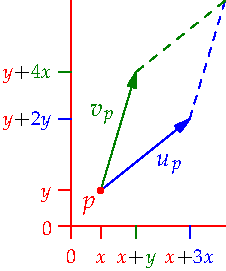
\includegraphics{forms-para}
	\end{minipage}
\end{example}

Recall that determinants change sign if you switch its rows or columns, and that they are linear functions of both their rows and columns. This has two consequences for $\alpha\wedge\beta$.

\begin{lemm}{}{wedge2}
	\exstart (Columns) \ At each $p\in U$, a wedge product of 1-forms is an \emph{alternating, bilinear function} $\alpha\wedge\beta:T_p\R^n\times T_p\R^n\to \R$: given vector fields $u,v,w$ and functions $f,g:U\to\R$,
	\begin{gather*}
		\alpha\wedge\beta\bigl(v,u\bigr)=-\alpha\wedge\beta\bigl(u,v\bigr) \tag{alternating}\\[5pt]
		\alpha\wedge\beta\bigl(fu+gv,w\bigr)=f\,\alpha\wedge\beta\bigl(u,w\bigr)+g\,\alpha\wedge\beta\bigl(v,w\bigr) \tag{linear in 1\st\ slot}
	\end{gather*}
	\begin{enumerate}\setcounter{enumi}{1}
	  \item (Rows) \ Wedge products are alternating and addition distributes over $\wedge$
	  \begin{gather*}
	  	\beta\wedge\alpha=-\alpha\wedge\beta\quad \text{and}\quad \alpha\wedge\alpha=0 \tag{alternating}\\
			(\alpha+\gamma)\wedge\beta=\alpha\wedge\beta+\gamma\wedge\beta \tag{distributivity in 1\st\ slot}
	  \end{gather*}
	\end{enumerate}
	Linearity/distributivity in the second slot is similar in both cases.
\end{lemm}

The linearity and alternating properties tell us that every wedge product of 1-forms on $\R^2$ may be written
\[
	\alpha\wedge\beta=\bigl(a_1\,\dx+a_2\,\dy\bigr)\wedge\bigl(b_1\,\dx+b_2\,\dy\bigr) =(a_1b_2-a_2b_1)\,\dx\wedge\dy
\]
Notice the determinant again!
\smallbreak

For higher order forms, we extend the same approach.

\begin{defn}{}{kform}
	The \emph{wedge product} of 1-forms $\alpha_1,\ldots,\alpha_k$ on $U\subseteq\R^n$ takes $k$ \emph{vector fields} and returns a \emph{smooth function}:\vspace{-5pt}
	\[
		\alpha_1\wedge\cdots\wedge\alpha_k\bigl(v_1,\ldots,v_k\bigr)=
		\scalebox{0.8}{$
			\begin{vmatrix}
				\alpha_1(v_1)&\cdots&\alpha_1(v_k)\\
				\vdots&\ddots&\vdots\\
				\alpha_k(v_1)&\cdots&\alpha_k(v_k)
			\end{vmatrix}
		$}:U\to\R\vspace{-5pt}
	\]
	Let $x_1,\ldots,x_n$ be co-ordinates on $U$. A \emph{$k$-form} on $U$ (alternating form of degree $k$) is an expression
	\[
		\alpha=\sum a_I\,\dx_{i_1}\wedge\cdots\wedge\dx_{i_k},\quad a_I:U\to\R\text{ smooth}
	\]
	where we sum over all \emph{increasing multi-indices} $I=\{i_1<i_2<\cdots< i_k\}\subseteq\{1,2,\ldots,n\}$ of length $k$.\smallbreak
	The \emph{wedge product} of a $k$-form $\alpha$ and an $l$-form $\beta$ is the $(k+l)$-form 
	\[
		\alpha\wedge \beta=\sum_{I,J}a_Ib_J\,\dx_{i_1}\wedge\cdots\wedge\dx_{i_k}\wedge\dx_{j_1}\wedge\cdots\wedge\dx_{j_l}
	\]
	where the 1-forms $\dx$ may be rearranged/cancelled using the alternating property (Lemma \ref{lemm:wedge2}.2).
\end{defn}

By convention, a 0-form is a smooth function $f:U\to\R$, whose wedge product with anything is pointwise multiplication. At each point $p\in U$, the $k$-forms comprise the vector space of alternating multilinear maps with basis $\{\dx_{i_1}\wedge\cdots\wedge\dx_{i_k}:i_1<\cdots<i_k\}$ and dimension $\binom nk=\frac{n!}{k!(n-k)!}$.\smallbreak

In this course we'll never have reason to work in more then three dimensions!\smallbreak


\begin{minipage}[t]{0.44\linewidth}\vspace{0pt}
The table describes all $k$-forms in 2 and 3 dimensions written in standard co-ordinates.\smallbreak
Analogous to Example \ref{ex:areaform}, $\dx\wedge\dy\wedge\dz$ is the \emph{standard volume form} on $\R^3$.
\end{minipage}\hfill\begin{minipage}[t]{0.52\linewidth}\vspace{0pt}
\flushright$\begin{array}{@{}c||c|c@{}}
	k&\R^2&\R^3\\\hline\hline
	0&\text{function }f&f\\\hline
	1&f\,\dx+g\,\dy & f\,\dx+g\,\dy+h\,\dz\\\hline
	2&f\,\dx\wedge\dy&f\,\dx\wedge\dy+g\,\dx\wedge\dz +h\,\dy\wedge\dz\\\hline
	3&\text{None}&f\,\dx\wedge\dy\wedge\dz\\\hline
	4+&\text{None}&\text{None}
\end{array}$
\end{minipage}


\begin{examples}{}{}
	\exstart Given 1-forms $\alpha=2\,\dx-3x\,\dy$ and $\beta=y^2\,\dx+y\,\dy$ on $\R^2$,
	\begin{align*}
		\alpha\wedge\beta&=(2\,\dx-3x\,\dy)\wedge\bigl(y^2\,\dx+y\,\dy\bigr)\\
		&=2y^2\,\dx\wedge\dx +2y\,\dx\wedge\dy -3xy^2\,\dy\wedge\dx -3xy\,\dy\wedge\dy\\
		&=\bigl(2y-3xy^2\bigr)\,\dx\wedge\dy
	\end{align*}
	
	\begin{enumerate}\setcounter{enumi}{1}
		\item Given the 1-forms $\alpha=\dx+2\,\dy+x\,\dz$ and 2-form $\beta=3z\,\dx\wedge\dy-\dy\wedge\dz$ on $\R^3$, the wedge product $\alpha\wedge\beta$ is the 3-form
		\begin{align*}
			\alpha\wedge\beta&=\dx\wedge(-\dy\wedge\dz)+3xz\,\dz\wedge\dx\wedge\dy\\
			&=(3xz-1)\,\dx\wedge\dy\wedge\dz
		\end{align*}
		Note how $\dz\wedge\dx\wedge\dy=-\dx\wedge\dz\wedge\dy=\dx\wedge\dy\wedge\dz$ requires \emph{two} swaps, so the sign is ultimately unchanged!
	\end{enumerate}
\end{examples}



\begin{lemm}{}{}
	For any forms $\alpha,\beta$,
	\[
		\beta\wedge\alpha=(-1)^{\deg\alpha\deg\beta}\alpha\wedge\beta
	\]
	where $\deg\alpha=k$ means that $\alpha$ is a $k$-form.
\end{lemm}


This is true by definition when $\alpha,\beta$ are 1-forms, and trivially true when $\alpha$ is a 0-form. Check the previous examples to make sure they agree.


\begin{example}{Polar co-ordinates}{polarcvar}
	Changing to polar co-ordinates, the standard area form on $\R^2$ becomes
	\[
		\dx\wedge\dy =(\cos\theta\,\dr-r\sin\theta\,\dth)\wedge (\sin\theta\,\dr+r\cos\theta\,\dth)=r\,\dr\wedge\dth
	\]
	This should remind you of change of variables in integration: if $f(x,y)=g(r,\theta)$, then
	\[
		\int f(x,y)\dx\dy=\int g(r,\theta)r\,\dr\dth
	\]
\end{example}

The example illustrates one of the advantages of forms: change of variables (Jacobians) are built in! %We won't have much need to integrate 2- and 3-forms in this course, though if you continue your studies of differential geometry\ldots


\boldinline{The Exterior Derivative}

Just as with functions, we can apply `$\D$' to forms.

\begin{defn}{}{}
	The \emph{exterior derivative} of a $k$-form $\alpha=\sum a_I\,\dx_{i_1}\wedge\cdots\wedge\dx_{i_k}$ is the $(k+1)$-form
	\[
		\D\alpha=\sum \D a_I\wedge\dx_{i_1}\wedge\cdots\wedge\dx_{i_k}
	\]
	where $\D a_I=\sum_j \partials[a]{x_j}\,\dx_j$ is the usual exterior derivative of a function (Definition \ref{defn:extderiv}).
\end{defn}

\begin{example}{}{formdiff}
	In $\R^3$, let $\alpha=xy^2z\,\dx-xz\,\dz$. Then
	\begin{align*}
		\D\alpha&=\D(xy^2z)\wedge\dx-\D(xy)\wedge\dz\\
		&=(\textcolor{blue}{y^2z\,\dx}+2xyz\,\dy+xy^2\,\dz)\wedge\dx -(z\,\dx+\textcolor{blue}{x\,\dz})\wedge\dz\\
		&=-2xyz\,\dx\wedge\dy -(xy^2+z)\,\dx\wedge\dz
	\end{align*}
	Since $\dx\wedge\dx=0=\dz\wedge\dz$, there was no need to write the \textcolor{blue}{blue} terms.
\end{example}


\begin{thm}{}{dsquared}
	Let $\alpha,\beta$ be forms:
	\begin{enumerate}
	  \item $\D(\alpha+\beta)=\D\alpha+\D\beta$\quad ($\alpha,\beta$ must have the same degree)
	  \item $\D(\alpha\wedge\beta)=\D\alpha\wedge\beta+(-1)^{\deg\alpha}\alpha\wedge\D\beta$
	  \item $\D(\D\alpha)=0$. This is often written\footnotemark\  $\D^2\alpha=0$, or just $\D^2=0$.
	\end{enumerate}
\end{thm}


\footnotetext{A $k$-form $\alpha$ is \emph{closed} if $\D\alpha=0$, and \emph{exact} if $\exists\beta$ such that $\alpha=\D\beta$. The result says that every exact form is closed.}

\goodbreak

\begin{example*}{\ref*{ex:formdiff} cont}{}
	We verify that $\D^2\alpha=0$:
	\begin{align*}
		\D(\D\alpha)&=\D(-2xyz)\wedge\dx\wedge\dy -\D(xy^2+z)\wedge\dx\wedge\dz\\
		&=-2xy\,\dz\wedge\dx\wedge\dy -2xy\,\dy\wedge\dx\wedge\dz =0
	\end{align*}
\end{example*}

\begin{proof}
	This is very easy to prove explicitly for the only forms we'll ever see (up to 3-forms in $\R^3$). Here are general arguments that work in any dimension.\smallbreak
	For simplicity of notation, write $\dx_I=\dx_{i_1}\wedge\dots\wedge\dx_{i_k}$, whenever $I=\{i_1<\cdots<i_k\}$. Then
	\[
		\D(\alpha+\beta)=\sum_I\D a_I\wedge\dx_I+\D b_I\wedge\dx_I =\sum_I(\D a_I+\D b_I)\wedge\dx_I =\D\alpha+\D\beta
	\]
	Part 2 is an exercise. For part 3, we extend Exercise \ref*{sec:1form}.\ref{exs:exactclosed} which in fact shows that $\D^2f=0$ for any function (0-form) 
	\begin{align*}
		\D(\D\alpha)&=\D\sum_I\D a_I\wedge\dx_I =\D\sum_{j\not\in I}\partials[a_I]{x_j}\,\dx_j\wedge\dx_I =\sum_{i,j\not\in I}\partials[^2a_I]{x_ix_j}\,\dx_i\wedge\dx_j\wedge\dx_I \\
		&=\sum_{i<j\not\in I}\left[\partials[^2a_I]{x_ix_j}-\partials[^2a_I]{x_jx_i}\right]\dx_i\wedge\dx_j\wedge\dx_I =0
	\end{align*}
	since mixed partial derivatives commute.
\end{proof}



\boldsubsubsection{A New Take on Vector Calculus}

The standard vector calculus operations of div, grad and curl in $\E^3$ are closely related to the exterior derivative. For instance, compare the curl of a vector field $\vv=a_1\vi+a_2\vj+a_3\vk$ with the exterior derivative of the 1-form $\alpha=a_1\,\dx+a_2\,\dy+a_3\,\dz$:
\begin{gather*}
	\nabla\times\vv=
	\threevec{\partials{x}}{\partials{y}}{\partials{z}}\times\threevec{a_1}{a_2}{a_3}
	=\left(\partials[a_3]{y}-\partials[a_2]{z}\right)\vi+ \left(\partials[a_1]{z}-\partials[a_3]{x}\right)\vj+ \left(\partials[a_2]{x}-\partials[a_1]{y}\right)\vk\\
	\D\alpha=\left(\partials[a_3]{y}-\partials[a_2]{z}\right)\,\dy\wedge\dz +\left(\partials[a_1]{z}-\partials[a_3]{x}\right)\,\dz\wedge\dx +\left(\partials[a_2]{x}-\partials[a_1]{y}\right)\,\dx\wedge\dy
\end{gather*}
Comparing coefficients gives part of the dictionary for comparing forms and traditional vector fields.
\[
	\xymatrix{
		%\xymatrixcolsep{-10pt}\text{\bf Forms} && \text{\bf Traditional vector fields}\\
		\text{function }f \ar@{|->}[d]^{\D} & \longleftrightarrow & \text{function }f \ar@{|->}[d]^{\nabla}_{\text{grad}}\\
		a_1\,\dx+a_2\,\dy+a_3\,\dz \ar@{|->}[d]^{\D} & \longleftrightarrow & a_1\vi+a_2\vj+ a_3\vk \ar@{|->}[d]^{\nabla\times}_{\text{curl}}\\
		b_1\,\dy\wedge\dz+b_2\,\dz\wedge\dx+b_3\,\dx\wedge\dy \ar@{|->}[d]^{\D} & \longleftrightarrow & b_1\vi+b_2\vj+b_3\vk \ar@{|->}[d]^{\nabla\cdot}_{\text{div}}\\
		c\,\dx\wedge\dy\wedge\dz & \longleftrightarrow & \text{function }c
	}
\]
The exterior derivative $\D$ is div, grad and curl all in one tidy package! Moreover:

\begin{itemize}
  \item The identity $\D^2=0$ translates to two familiar results from vector calculus:
  \[
  	\nabla\times(\nabla f)=\V0\quad\text{and}\quad\nabla\cdot(\nabla\times\vv)=0
  \]
  
  \item Under the above identification, the wedge product of 1-forms corresponds to the cross product, and the wedge product of a 1-form and a 2-form to the dot product. Various identities may be obtained this way: for instance, if $\alpha$ is a 1-form, then
  \[
  	\D(f\alpha)=\df\wedge\alpha+f\D\alpha \quad\longleftrightarrow
\quad\nabla\times f\vv=\nabla f\times\vv+f\nabla\times\vv
	\]
	 	
  \item Changes of co-ordinates are built into forms (e.g.\ Example \ref{ex:polarcvar}).
  
  \item The exterior derivative and wedge product apply in any dimension, thus extending standard vector calculus and the cross product to arbitrary dimensions. 
\end{itemize}

% The exterior derivative and the wedge product are host of useful operators in one!\smallbreak

None of what we've done in this chapter is strictly necessary for the analysis of surfaces in $\E^3$. However, forms are the language of modern differential geometry (and other things besides) and it is easier to meet them first in a familiar setting. And if you want to do higher-dimensional geometry (e.g.,\ general relativity), this new language becomes almost essential.



\begin{exercises}
	\exstart Compute $\alpha(u,v)$, given $\alpha=\dx\wedge\dy+z\,\dy\wedge\dz$, \ $u=\partials{x}-\partials{z}$ and $v=y\partials{y}+\partials{z}$.\vspace{-3pt}
%  Now,
% \begin{gather*}
% (\dx_1\wedge\dx_2)(u,v)=
% \begin{vmatrix}
% \dx_1(u)&\dx_1(v)\\
% \dx_2(u)&\dx_2(v)
% \end{vmatrix}
% =x_2,\qquad (\dx_2\wedge\dx_3)(u,v)=x_2\\
% \therefore\beta(u,v)=x_2(1+x_3)
% \end{gather*}

	\begin{enumerate}\setcounter{enumi}{1}
	  \item Let $\alpha=y^2\,\dx\wedge\dz-\dy\wedge\dz$ and $u=x\partials x+xy\partials y-\partials z$ and $v=-y\partials x+y^3\partials y$.
		\begin{enumerate}
		  \item Compute $\alpha(u,v)$.
		  \item Find the 3-form $\D\alpha$.
		\end{enumerate}
		
		
		\item Given $s=x^2-y^2$ and $t=2xy$, compute $\ds\wedge\dt$ in terms of $\dx\wedge\dy$
		
		
		\item Revisit Lemma \ref{lemm:wedge2}. State what it means for a wedge product of 1-forms $\alpha\wedge\beta$ to be linear in the second slot.
		
		
		\item Let $f,g$ be functions and consider the 1-form $\alpha=g\,\df$. Show that $\alpha\wedge\D\alpha=0$. Can the 1-form $\dx+y\,\dz$ be written in the form $g\,\df$?
		
		
		\item\begin{enumerate}
		  \item Check the claim that the wedge product of 1-forms on $\R^3$ corresponds to the cross product.
		  \item Suppose $\alpha$ is a 2-form on $\R^3$. To what vector calculus identity does $\D(f\alpha)=\df\wedge\alpha+f\D\alpha$ correspond?
		  \item State an expression using forms, $\D$ and $\wedge$ which corresponds to the vector calculus identity
		  \[
		 		\nabla\cdot(\vu\times\vv) =(\nabla\times\vu)\cdot\vv-\vu\cdot(\nabla\times\vv)
		 	\]
		\end{enumerate}
		
		
		\item Let $r,\theta,\phi$ be the spherical polar co-ordinate system in Exercise \ref*{sec:vfield}.\ref{exs:spherical}. Show that 
		\[
			\dx\wedge\dy\wedge\dz=r^2\cos\phi\,\dr\wedge\dth\wedge\D\phi
		\]
	
	% 	\item grad in polar co-ords?
	% 
	% 	\begin{gather*}
	% 	\df=\partials[f]{r}\dr+\partials[f]{\theta}\dth =\frac{f_r}r(x\,\dx+y\,\dy) + \frac{f_\theta}{r^2}(-y\,\dx+x\,\dy)\\
	% 	\implies \nabla f=f_r\twovec{\cos\theta}{\sin\theta}+\frac{f_\theta}r\twovec{-\sin\theta}{\cos\theta} =f_r\,\hat\vr+\frac{f_\theta}r\hat{\pmb{\theta}}
	% 	\end{gather*}
	
		\goodbreak
	
		\item A 2-form is \emph{decomposable} if it can be written as a wedge product $\alpha\wedge\beta$ for some 1-forms $\alpha,\beta$.
		\begin{enumerate}
		  \item Show that every 2-form on $\R^3$ is decomposable.
		  
		  \item If $w,x,y,z$ are co-ordinates on $\R^4$, show that the 2-form $\dw\wedge\dx+\dy\wedge\dz$ is \emph{not} decomposable.\par
		  (\emph{Hint: if a 2-form $\gamma$ is decomposable, what is $\gamma\wedge\gamma$?})
		\end{enumerate}
		
	
		
		\item (Hard)\lstsp Suppose $\alpha,\beta$ are forms, sketch an argument for why
		\[
			\alpha\wedge\beta=(-1)^{\deg\alpha\deg\beta}\beta\wedge\alpha
		\]
		Now prove that
		\[
			\D(\alpha\wedge\beta)=\D\alpha\wedge\beta+(-1)^{\deg\alpha}\alpha\wedge\D\beta
		\]
		
		
		\item\label{exs:liebracketdalpha} (Hard)\lstsp Given vector fields $u,v$, their \emph{Lie bracket} $[u,v]$ is the vector field such that
		\[
			[u,v][f]:=u\bigl[v[f]\bigr] -v\bigl[u[f]\bigr]
		\]
		for all functions $f$.
		\begin{enumerate}
		  \item Compute $[u,v][f]$ where $u=3x\partials x+\partials y$ and $v=\partials x-x\partials y$ and $f(x,y)=x^2y$.
		  
		  \item If $u=\sum u_j\partials{x_j}$ and $v=\sum v_k\partials{x_k}$, show that $[u,v]$ really is a vector field by explicitly computing $[u,v][f]$ in the form $\sum c_j\partials[f]{x_j}$: how do the coefficients $c_j$ of the vector field $[u,v]$ depend on those of $u,v$? Find the \emph{field} $[u,v]$ when $u,v$ are as in part (a).
		  
		  \item If $\alpha$ is a 1-form and $u,v$ are vector fields, prove that
		  \[
		  	\D\alpha\bigl(u,v\bigr)=u\bigl[\alpha(v)\bigr]-v\bigl[\alpha(u)\bigr]-\alpha\bigl([u,v]\bigl)
		  \]
		  \emph{This provides a co-ordinate-free definition of $\D\alpha$; similar expressions exist for $k$-forms}\par
		  (\emph{Hint: Write everything out as sums over $j,k$ so that all differentiations of scalars are with respect to the single variable $x_k$; now compare!})
		\end{enumerate}
		
	\end{enumerate}
\end{exercises}

